
\normalsize

\section*{APPENDIX A: Experimental Details}

\minihead{Microbenchmark experiment description} We implemented traditional two-phase locking and an optimized variant of two-phase locking on the experimental prototype described in Section~\ref{sec:evaluation}.

In two-phase locking, each client acquires locks one at a time, requiring a full round trip time (RTT) for every lock request. For an $N$ item transaction, locks are held for $2N+1$ message delays (the $+1$ is due to broadcasting the unlock/commit command to the participating servers).

Our optimized two-phase locking only uses one message delay (half RTT) to perform each lock request: the client specifies the entire set of items it wishes to modify at the start of the transaction (in our implementation, the number of items in the transaction and the starting item ID), and, once a server has updated its respective item, the server forwards the remainder of the transaction to the server responsible for the next write in the transaction. For an $N$-item transaction, locks are only held for $N$ message delays (the final server both broadcasts the unlock request to all other servers and also notifies the client), while a $1$-item transaction does not require distributed locking.

To avoid deadlock (which was otherwise common in this high-contention microbenchmark), our implementation totally orders any lock requests according to item and executes them sequentially (e.g., lock server $1$ then lock server $2$). Our implementation also piggybacks write commands along with lock requests, further avoiding message delays. Unlike the locking implementation used in Section~\ref{sec:evaluation}, since we are only locking one item per server, our microbenchmark code does not use a dynamic lock manager and instead associates a single lock with each item; this should further lower locking overheads.

On each server, our lock implementation uses Java \texttt{ReentrantLock}, which unfortunately means that, for all but $1$-item optimized 2PL, our implementation was unable to used fixed-size thread pools (in contrast with our Scala \texttt{Future}-based coordination-free runtime). Nevertheless, we do not believe that our locking implementation is the actual bottleneck in the distributed setting: coordination is.

We partitioned eight in-memory items (integers) across eight \texttt{cr1.8xlarge} Amazon EC2 instances with clients located on a separate set of \texttt{cr1.8xlarge} instances. Figure~\ref{fig:micro} reported in Section~\ref{sec:motivation} depicts results for the coordination-free implementation and the optimized two-phase locking case. Figure~\ref{fig:micro-all} in this second depicts all three algorithms. Unsurprisingly, two-phase locking performs worse than optimized two-phase locking, but both incur substantial penalties due to coordination delay over the network.

\begin{figure}
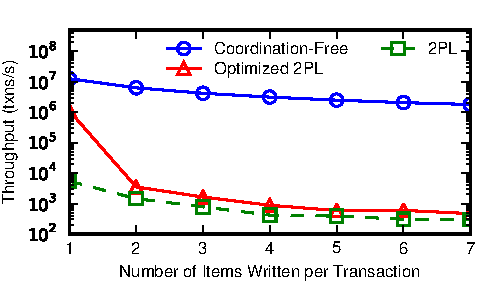
\includegraphics[width=\columnwidth]{figs/micro_thru_all.pdf}
\caption{Additional performance details for microbenchmark performance of conflicting and non-conflicting
  transactions.}
\label{fig:micro-all}
\end{figure}

\minihead{Trace-based simulation description} We simulate traditional two-phase commit and decentralized two-phase commit, using network models derived from existing studies. Our simulation is rather straightforward, but we make several optimizations to improve the throughput of each algorithm. First, we assume that transactions are pipelined, so that each server can \texttt{prepare} immediately after it has \texttt{commit}ted the prior transaction. Second, our pipelines are ideal in that we do not consider deadlock: only one transaction \texttt{prepare}s at a given time. Third, we do not consider the cost of local processing of each transaction: throughput is determined entirely by communication delay.

While this study is based solely on reported latencies, deployment
reports corroborate our findings. For example, Google's F1 uses
optimistic concurrency control via WAN with commit latencies of $50$
to $150$~ms. As the authors discuss, this limits throughput to between
$6$ to $20$ transactions per second per data
item~\cite{f1}. Megastore's average write latencies of $100$ to
$400$~ms suggest similar throughputs to those that we have
predicted~\cite{megastore}. Again, \textit{aggregate} throughput may
be greater as multiple 2PC rounds for disjoint sets of data items may
safely proceed in parallel. However, \textit{worst-case} access
patterns will indeed greatly limit scalability.

\section*{APPENDIX B: \iconfluence proof}

\begin{lemma}\label{lemma:force} 
Given a set of transactions $T$ and invariants $I$, a globally $I$-valid, coordination-free, transactionally available, and convergent system is able to produce any $I$-$T$-reachable state $S_i$.
 \end{lemma} \begin{proof}{Lemma~\ref{lemma:force}}
Let $\alpha_i$ represent a partially ordered sequence of transactions $T_i$ and merge procedure invocations $M_i$ (call this a \textit{history}) starting from $S_0$ that produces $S_i$,

We $\textsc{replay}$ the history $\alpha_i$ on a set of servers as follows. Starting from the initial state $S_0$, we traverse the partial order according to what amounts to a topological sort. Initially, we mark all operations (transactions or merges) in $\alpha_i$ as \textit{not done}. We begin by executing all transactions $T_i$ in $\alpha_i$ that have no predeceding operations in $\alpha_i$. For each transaction $t \in T_i$, we execute $t$ on a server that is unable to communicate with any other server. Upon transaction commit, we merge each replica's modifications into a separate server.  (Recall that, because $S_i$ is $I$-$T$-reachable, each transaction in $\alpha_i$ is an $I$-valid transformation and must either eventually commit or abort itself to preserve transactional availability, and, due to coordination-freedom, the result of the execution is dependent solely on its input---in this case, $S_0$.) We subsequently mark each $t \in T_i$ as \textit{done} in $\alpha_0$ and denote the resulting server as $s_t$.\footnote{Recall from Section~\ref{sec:model} that we consider arbitrary sets of servers. We could likely (at least in certain cases) be more parsimonius with our use of servers in this proof at some cost to complexity.} 

Next, we repeatedly select an operation $o_i$ from $\alpha_i$ that is marked as \textit{not done} but whose preceding operations are all marked as \textit{done}.

If $o_i$ is a transaction with preceding operation $o_j$ on corresponding server $s_j$, we partition $s_j$ and $s_i$ and another server containing state $S_0$ such that $s_j$ and $s_i$ can communicate with each other but cannot communicate with any other server. Under convergent execution, $s_j$ and $s_i$ must eventually contain the same state, merged to $s_j$ (given that $s_j \sqcup S_0$ is defined in our model to be $s_j$). Following convergence, we partition $s_j$ and $s_i$ so they cannot communicate. We subsequently execute $o_i$ on $s_j$. Again, $o_i$ must either commit or abort itself to preserve transactional availability, and its behavior is solely dependent on its input due to coordination-freedom.

If $o_i$ is a merge procedure with preceding operations $o_j$ and $o_k$ on corresponding servers $s_j$ and $s_k$, we produce servers $s_{j'}$ and $s_{k'}$ as above, by partitioning $s_{j'}$ and $s_{j}$ and, respectively, $s_{k}$ and $s_{k'}$, waiting until convergence, then repartitioning each. Subsequently, we place $s_{j'}$ and $s_{k'}$ in the same partition, forcing the merge ($o_i$) of these states via the convergence requirement.

When all operations in $\alpha_i$ are marked as \textit{done}, the final operation we have performed will produce server containing state $S_i$. We have effectively (serially) traversed the history, inducing the series of transactions by triggering partitions while requiring commits due to transactional availability and merges due to our pair-wise convergence.
\end{proof}

We proceed to prove Theorem~\ref{theorem:necessary} from Section~\ref{sec:ic-result}.

\begin{proof}{Theorem~\ref{theorem:necessary}}
($\Leftarrow$) We begin with the simpler proof, which is by
  construction. Assume a set of transactions $T$ are \iconfluent with
  respect to an invariant $I$. Consider a system in which each server
  executes the transactions it receives against a replica of its current state and checks whether or not the resulting state is $I$-valid. If
  the resulting state is $I$-valid, the replica commits the
  transaction and its mutations to the state. If not, the replica
  aborts the transaction. Servers opportunistically exchange copies of
  their local states and merge them. No individual replica will
  install an invalid state upon executing transactions, and, because
  $T$ is \iconfluent under $I$, the merge of any two $I$-valid replica
  states from individual servers (i.e., $I$-$T$-reachable states) as
  constructed above is $I$-valid. Therefore, the converged database
  state will be $I$-valid. Transactional availability, convergence,
  and global $I$-validity are all maintained via coordination-free
  execution.

($\Rightarrow$) Assume a system $M$ guarantees globally $I$-valid
  operation for set of transactions $T$ and invariant $I$ with
  \cfreedom, transactional availability, and convergence, but $T$ is
  not $I$-confluent. Then there exist two $I$-$T$-reachable states $S_1$ and $S_2$ with common ancestor $I$-$T$-reachable state $S_a$ such that, by definition, $I(S_1)$ and $I(S_2)$ are true, but $I(S_1 \sqcup S_2)$ is false. \footnote{We may be able to apply Newman's
  lemma and only consider single-transaction divergence (in the case 
  of convergent and therefore ``terminating'' 
  executions)~\cite{obs-confluence,termrewriting}, but this is not 
  necessary for our results.\label{fn:newman-note}}

Consider two executions of system $M$, $\epsilon_1$ and $\epsilon_2$. In each execution, we begin by forcing $M$ to produce a server containing $S_c$ (via \textsc{replay} in Lemma~\ref{lemma:force}). In $\epsilon_1$, we subsequently \textsc{replay} the history $\alpha_1$ starting from $S_c$. In $\epsilon_2$, we subsequently \textsc{replay} the history $\alpha_2$ starting from $S_c$. Call $T_{f1}$ and $T_{f2}$ the final (set of) transactions that produced each of $S_1$ and $S_2$ (that is, the set of transactions in each execution that are not followed by any other transaction). Under $\alpha_1$ and $\alpha_2$, all transactions in each of $T_{f1}$ and $T_{f2}$ will have committed to maintain transactional availability, their end result will be equivalent to the result in $\alpha_1$ and $\alpha_2$ due to the coordination-freedom property, and $S_1$ and $S_2$ are both $I$-valid, by assumption.

We now consider a third execution, $\alpha_3$. $\alpha_3$ proceeds to independently \textsc{replay} $\alpha_1$ and $\alpha_2$ but does not execute or proceed further in the partial order than any element of $T_{f1}$ or $T_{f2}$; we consider these specially:

Once $\alpha_3$ has forced $M$ to \textsc{replay} other operations, we force it to \textsc{replay} these final operations beginning from $T_{f1}$ and $T_{f2}$. If we \textsc{replay} these transactions and $M$ commits them, we can \textsc{replay} the remainder of the operations in $\alpha_1$ and $\alpha_2$. In this case, due to the coordination-freedom property, $M$ will produce two servers $s_i$ and $s_j$ containing states $S_1$ and $S_2$. When we partition $s_i$ and $s_j$ such that they can communicate with each other but cannot communicate with any other servers, $s_i$ and $s_j$ must eventually converge, violating global $I$-validity. On the other hand, if $M$ aborts one or more of the transactions in $T_{f1}$ and $T_{f2}$, $M$ will not produce $s_i \sqcup s_j$, but, from the perspective of each server $s_{p1}$ executing a transaction in $T_{f1}$, this execution is indistinguishable from $\alpha_1$, and, from the perspective of each server $s_{p2}$ executing a transaction in $T_{f2}$, is indistinguishable from $\alpha_2$, a contradiction.

Therefore, to preserve transactional availability, $M$ must sacrifice one of global validity (by allowing the invalid merge), convergence (by never   merging), or \cfreedom (by requiring changes to transaction behavior).
\end{proof}

\section*{APPENDIX C: \iconfluence Analysis}

In this section, we more formally demonstrate the \iconfluence of invariants and operations discussed in Section~\ref{sec:merge}. Our goals in this section are two-fold. First, we have found the experience of formally proving \iconfluence to be instructive in understanding these combinations (beyond less formal arguments made in the body text for brevity and intuition). Second, we have found \iconfluence proofs to take on two general structures that, via repetition and in and variations below, may prove useful to the reader. In particular, the structure of our \iconfluence proofs takes one of two forms:

\begin{itemize}

\item To show a set of transactions are not \iconfluent with respect to an invariant $I$, we use proof by counterexample: we present two $I$-$T$-reachable states with a common ancestor that, when merged, are not $I$-valid. 

\item To show a set of transactions are \iconfluent with respect to an invariant $I$, we use proof by contradiction: we show that, if a state $S$ is not $I$-valid, merging two $I$-$T$-reachable states with a common ancestor state to produce $S$ implies either one or both of $S_1$ or $S_2$ must not be $I$-valid.

\end{itemize}

These results are not exhaustive, and there are literally infinite combinations of invariants and operations to consider. Rather, the seventeen examples below serve as a demonstration of what can be accomplished via \iconfluence analysis.

Notably, the negative results below use fairly simple histories consisting of a single transaction divergence. As we hint in Footnote~\ref{fn:newman-note}, it is possible that a large class of relevant invariant-operation pairs only depend on single-transaction divergence. Nevertheless, we decided to preserve the more general formulation of \iconfluence (accounting for arbitrary $I$-$T$-reachable states) to account for more pathological (perhaps less realistic, or, if these results are any indication, less commonly encountered) behaviors that only arise during more complex divergence patterns.

We introduce additional formalism as necessary. To start, unless otherwise specified, we use the set union merge operator. We denote version $i$ of item $x$ as $x_i$ and a write of version $x_i$ with value $v$ as $w(x_i=v)$.

\begin{claim}[Writes are \iconfluent with respect to per-item equality constraints]
\label{claim:eq-proof}
Assume writes are not \iconfluent with respect to some per-item equality constraint $i=c$, where $i$ is an item and $c$ is a constant. By definition, there must exist two $I$-$T$-reachable states $S_1$ and $S_2$ with common ancestor state such that $I(S_1) \rightarrow true$ and $I(S_2) \rightarrow true$ but $I(S_1) \sqcup S_2) \rightarrow false$; therefore, there exists a version $i_n$ in $S_1 \sqcup S_2$ such that $i_n \neq c$, and, under set union, $i_n \in S_1$, $i_n \in S_2$, or both. However, this would imply that $I(S_1) \rightarrow false$ or $I(S_2) \rightarrow false$ (or both), a contradiction.
\end{claim} 

\begin{claim}[Writes are \iconfluent with respect to per-item inequality constraints] \label{claim:neq} The proof follows almost identically to the proof of Claim, but for an invariant of the form $i\neq c$~\ref{claim:eq-proof}.  \end{claim}

\begin{claim}[Writing arbitrary values is not \iconfluent with respect to multi-item uniqueness constraints]
\label{claim:sunique}
Consider the following transactions:
\begin{align*}
T_{1u}&\coloneqq w(x_a=v);~commit\\
T_{2u}&\coloneqq w(x_b=v);~commit
\end{align*}
and uniqueness constraint on records:
$$I_u(D) = \{\textrm{values in D are unique}\}$$
Now, an empty database trivially does not violate uniqueness constraints ($I_u(D_s=\{\})\rightarrow true$), and adding individual versions to the separate empty databases is also valid:
\begin{align*}
T_{1u}(\{\})&=\{x_a=v\},~I_u(\{x_a=v\}) \rightarrow true\\
T_{2u}(\{\})&=\{x_b=v\},~I_u(\{x_b=v\}) \rightarrow true
\end{align*}
However, merging these states results in invalid state:
$$I_u(\{x_a=v\}\sqcup \{x_b=v\} = \{x_a=v, x_b=v\}) \rightarrow false$$
Therefore, $\{T_{1u}, T_{2u}\}$ is not \iconfluent under $I_s$.
\end{claim} 

For the next proof, we consider a model as suggested in Section~\ref{sec:bcc-practice} where replicas are able to generate unique (but not arbitrary (!)) IDs (in the main text, we suggested the use of a replica ID and sequence number). In the following proof, to account for this non-deterministic choice of unique ID, we introduce a special $nonce()$ function and require that, $nonce()$ return unique values for each replica; that is, $\sqcup$ is not defined for replicas on which independent invocations of $nonce()$ return the same value.

\begin{claim}[Assigning values by $nonce()$ is \iconfluent with respect to multi-item uniqueness constraints]
\label{claim:nunique}

Assume that assigning values by $nonce()$ is not \iconfluent with respect to some multi-item uniqueness invariant:
$$I(D) = \forall c \in dom(D), \{|\{x \in D \mid x = c\}| \leq 1 \}$$
By definition, there must exist two $I$-$T$-reachable states with a common ancestor reached by executing nonce-generating transactions (of the form $T_i=[w(x_i = nonce())]$), $S_1$ and $S_2$ such that $I(S_1) \rightarrow true$ and $I(S_2) \rightarrow true$ but $I(S_1 \sqcup S_2) \rightarrow false$.

Therefore, there exist two versions $i_a, i_b$ in $S_1 \sqcup S_2$ such that $i_a$ and $i_b$ (both generated by $nonce()$) are equal in value. Under set union, this means $i_a \in S_1$ and $i_b \in S_2$ ($i_a$ and $i_b$ both cannot appear in $S_1$ or $S_2$ since it would violate those states' $I$-validity). Because replica states grow monotonically under set merge and $S_1$ and $S_2$ differ, they must be different replicas. But $nonce()$ cannot generate the same values on different replicas, a contradiction. \end{claim}

\begin{claim}[Writing arbitrary values are not \iconfluent with respect to sequentiality constraints]
\label{claim:nseq-insert}
Consider the following transactions:
\begin{align*}
T_{1s}&\coloneqq w(x_a=1);~commit\\
T_{2s}&\coloneqq w(x_b=3);~commit
\end{align*}
and the sequentiality constraint on records:
$$I_s(D) =\{max(r\in D)-min(r\in D) = |D|+1\} \vee \{|D|=0\}$$
Now, $I_s$ holds over the empty database ($I_s(\{\}) \rightarrow true$), while inserting sequential new records into independent, empty replicas is also valid:
\begin{align*}
T_{1s}(\{\})&=\{x_a=1\},~I_u(\{x_a=1\} \rightarrow true\\
T_{2s}(\{\})&=\{x_b=3\},~I_u(\{x_b=3\} \rightarrow true
\end{align*}
However, merging these states results in invalid state:
$$I_s(\{x_a=1\}\sqcup \{x_b=3\} = \{x_a=1, x_b=3\}) \rightarrow false$$
Therefore, $\{T_{1s}, T_{2s}\}$ is not \iconfluent under $I_s$.
\end{claim}

To discuss foreign key constraints, we need some way to \textit{refer} to other records within the database. There are a number of ways of formalizing this; we are not picky and, here, refer to a field $f$ within a given version $x_i$ as $x_i.f$.

\begin{claim}[Insertion is \iconfluent with respect to foreign key constraints]
\label{claim:fk-insert}
  Assume that inserting new records is not \iconfluent with respect to some foreign key constraint $I(D) = \{\forall r_f \in D$ such that $r_f.g \neq null$, $\exists r_t \in D$ such that $r_f.g = r_t.h\}$ (there exists a foreign key reference between fields $g$ and $h$). By definition, there must exist two $I$-$T$-reachable states $S_1$ and $S_2$ with a common ancestor reachable by executing transactions performing insertions such that $I(S_1) \rightarrow true$ and $I(S_2) \rightarrow true$ but $I(S_1 \sqcup S_2) \rightarrow false$; therefore, there exists some version $r_1 \in S_1 \sqcup S_2$ such that $r_1.f \neq null$ but $\nexists r_2 \in S_1 \sqcup S_2$ such that $r_1.g = r_2.h$. Under set union, $r_1$ must appear in either $S_1$ or $S_2$ (or both), and, for each set of versions in which it appears, because $S_1$ and $S_2$ are both $I$-valid, they must contain an $r_3$ such that $r_1.f = r_3.h$. But, under set union, $r_3.h$ should also appear in $S_1 \sqcup S_2$, a contradiction.
\end{claim}

For simplicity, in the following proof, we assume that deleted elements remain deleted under merge. In practice, this can be accomplished by tombstoning records and, if required, using counters to record the number of deletions and additions~\cite{crdt}. We represent a deleted version $x_d$ by $\neg x_b$.

\begin{claim}[Concurrent deletion and insertion is not \iconfluent with respect to foreign key constraints]
\label{claim:fk-delete}
 Consider the following transactions:
\begin{align*}
T_{1f}&\coloneqq w(x_a.g=1);~commit\\
T_{2f}&\coloneqq delete(x_b);~commit
\end{align*}
and the foreign key constraint:
$$I_f(D) = \{\forall r_f \in D, r_f.g \neq null,~\exists r_t \in D \suchthat \neg r_t \notin D \mathand r_f.g = r_t.h\}$$
Foreign key constraints hold over the initial database $S_i=\{x_b.h=1\}$ ($I_u(S_i) \rightarrow true$) and on independent execution of $T_a$ and $T_b$:
\begin{align*}
T_{1f}(\{x_b.h=1\})&=\{x_a.g=1, x_b.h=1\},~I_f(\{x_a=1\}) \rightarrow true\\
T_{2f}(\{x_b.h=1\})&=\{x_b.h=1, \neg {x_b}\}~I_f(\{x_b.h=1, \neg {x_b}\}) \rightarrow true
\end{align*}
However, merging these states results in invalid state: 
$$I_f(\{x_a.g=1\}\sqcup \{x_b.h=1, \neg {x_b}\}) \rightarrow false$$
Therefore, $\{T_{1f}, T_{2f}\}$ is not \iconfluent under $I_f$.\end{claim}

We denote a casading delete of all records that reference field $f$ with value $v$ ($v$ a constant) as $cascade(f=v)$.

\begin{claim}[Cascading deletion and insertion are \iconfluent with respect to foreign key constraints]
\label{claim:fk-cascade}
Assume that cacading deletion and insertion of new records are not \iconfluent with respect to some foreign key constraint $I(D) = \{\forall r_f \in D$ such that $r_f.g \neq null$, $\exists r_t \in D$ such that $r_f.g = r_t.h$ if $cascade(h=r_f.g \neq v)\}$ (there exists a foreign key reference between fields $g$ and $h$ and the corresponding value for field $h$ has not been deleted-by-cascade). By definition, there must exist two $I$-$T$-reachable states $S_1$ and $S_2$ with common ancestor reachable by performing insertions such that $I(S_1) \rightarrow true$ and $I(S_2) \rightarrow true$ but $I(S_1 \sqcup S_2) \rightarrow false$; therefore, there exists some version $r_1 \in S_1 \sqcup S_2$ such that $r_1.f \neq null$ but $\nexists r_2 \in S_1 \sqcup S_2$ such that $r_1.g = r_2.h$. From the proof of Claim~\ref{claim:fk-insert}, we know that insertion is \iconfluent, so the absence of $r_2$ must be due to some cascading deletion. Under set union, $r_1$ must appear in exactly one of $S_1$ or $S_2$ (if $r_1$ appeared in both, there would be no deletion, a contradiction since we know insertion is \iconfluent). For the state $S_j$ in which $r_1$ does not appear (either $S_1$ or $S_2$), $S_j$ must include $cascade(h=r_1.g)$. But, if $cascade(h=r_1.g) \in S_j$, $cascade(h=r_1.g)$ must also be in $S_i \sqcup S_j$, a contradiction and so $S_i \sqcup S_j \rightarrow true$, a contradiction.
\end{claim}

We define a ``consistent'' secondary index invariant as requiring that, when a record is visible, its secondary index entry should also be visible. This is similar to the guarantees provided by Read Atomic isolation~\cite{ramp-txns}. For simplicity, in the following proof, we only consider updates to a single indexed attribute $attr$, but the proof is easily generalizable to multiple index entries, insertions, and deletion via tombstones. We use last-writer wins for index entries.

\begin{claim}[Updates are \iconfluent with respect to consistent secondary indexing] \label{claim:indexing}
  Assume that updates to records are not \iconfluent with respect a secondary index constraint on attribute $attr$:\vspace{.5em}

\noindent $I(D) = \{\forall r_f \in D$ such that $r_f.attr \neq null$ and $f$ is the highest version of $r\in D$, $\exists r_{idx} \in D$ such that $r_f \in r_{idx}.entries$ (all entries with non-null $attr$ are reflected in the secondary index entry for $attr$)\vspace{.5em}

  Represent an update to record $r_x$ as $\{w(r_x)$ and, if $r_x.attr \neq null$, also $r_{idx}.entries.add(r_x)$, else $r_{idx}.entries.delete(r_x)\}$.\vspace{.5em}

  By definition, there must exist two $I$-$T$-reachable states $S_1$ and $S_2$ with common ancestors reachable by performing insertions $S_1$ and $S_2$ such that $I(S_1) \rightarrow true$ and $I(S_2) \rightarrow true$ but $I(S_1 \sqcup S_2) \rightarrow false$; therefore, there exists some version $r_1 \in S_1 \sqcup S_2$ such that $r_1.attr \neq null$ but $\nexists r_{idx} \in S_1 \sqcup S_2$ or $\exists r_{idx} \in S_1 \sqcup S_2$ but $r_1 \notin r_{idx}.entries$. In the former case, $r_{idx} \notin S_1$ or $S_2$, but $r_1 \in S_1$ or $r_1 \in S_2$, a contradiction. The latter case also produces a contradiction: if $r_1 \in S_1$ or $r_1 \in S_2$, it must appear in $r_{idx}$, a contradiction.  \end{claim}

In our formalism, we can treat materialized views as functions over database state $f(D) \rightarrow c$.

\begin{claim}[Updates are \iconfluent with respect to materialized view maintenance] The proof is relatively straightforward if we treat the materialized view record(s) $r$ as having a foreign key relationship to any records in the domain of the function (as in the proof of Claim~\ref{claim:fk-cascade} and recompute the function on update, cascading delete, and $\sqcup$.\end{claim}

For our proofs over counter ADTs, we represent increments of a counter $c$ by $inc_i(c)$, where $i$ is a distinct invocation, decrements of $c$ by $dec_i(c)$, and the value of $c$ in database $D$ as $val(c, D) = |\{j \mid inc_j(c) \in D\}| - |\{k \mid dec_k(c) \in D\}|$.

\begin{claim}[Counter ADT increments are \iconfluent with respect to greater-than constraints] \label{claim:ge-inc-adt}
Assume increments are not \iconfluent with respect to some per-counter greater-than constraint $I(D)=val(c, D) < k$, where $k$ is a constant. By definition, there must exist two $I$-$T$-reachable states $S_1$ and $S_2$ with common ancestor reachable by executing write transactions such that $I(S_1) \rightarrow true$ and $I(S_2) \rightarrow true$ but $I(S_1 \sqcup S_2) \rightarrow false$; therefore, $val(c, S_1 \sqcup S_2) \leq k$. However, this implies that $val(c, S_1) \leq k)$, $val(c, S_2$, or both, a contradiction.  \end{claim}

\begin{claim}[Counter ADT increments are not \iconfluent with respect to less-than constraints]
\label{claim:le-inc-adt}
Consider the following transactions:
\begin{align*}
T_{1i}&\coloneqq inc_1(c);~commit\\
T_{2i}&\coloneqq inc_2(c);~commit
\end{align*}
and the less-than inequality constraint:
$$I_i(D) = \{val(c, D) < 2\}$$
$I_i$ holds over the empty database state ($I_i(\{\}) \rightarrow true$) and when $T_a$ and $T_b$ are independently executed:
\begin{align*}
T_{1i}(\{\})&=\{inc_1(c)=1\},~I_i(\{inc_1(c)=1\}) \rightarrow true\\
T_{2i}(\{\})&=\{inc_2(c)\},~I_i(\{inc_2(c)\}) \rightarrow true
\end{align*}
However, merging these states results in invalid state:
$$I_u(\{inc_1(c)\}\sqcup \{inc_2(c)\}) \rightarrow false$$
Therefore, $\{T_{1i}, T_{2i}\}$ is not \iconfluent under $I_u$.
\end{claim}

\begin{claim}[Counter ADT decrements are not \iconfluent with respect to greater-than constraints] The proof is similar to the proof of Claim~\ref{claim:le-inc-adt}; substitute $dec$ for $inc$ and choose $I_i(D) = \{val(c,D) > -2\}$.  \end{claim}

\begin{claim}[Counter ADT decrements are \iconfluent with respect to less-than constraints] \label{claim:le-inc-adt} Unsurprisingly, the proof is almost identical to the proof of Claim~\ref{claim:ge-inc-adt}, but with $<$ instead of $>$ and $dec$ instead of $inc$. \end{claim}

We provide proofs for ADT lists; the remainder are remarkably similar. Our implementation of ADT lists in these proofs uses a lexicographic sorting of values to determine list order. Transactions add a version $v$ to list $l$ via $add(v,l)$ and remove it via $del(v,l)$ (where an item is considered contained in the list if it has been added more times than it has been deleted) and access the length of $l$ in database $D$ via $size(l) = |\{k \mid add(k, l) \in D\}|- |\{m \mid del(m, l) \in D\}|$ (note that $size$ of a non-existent list is zero).

\begin{claim}[Modifying a list ADT is \iconfluent with respect to containment constraints]
  Assume ADT list modifications are not \iconfluent with respect to some equality constraint $I(D)=\{add(k, l) \in D \wedge del(k, l) \notin D \}$ for some constant $k$. By definition, there must exist two $I$-$T$-reachable states $S_1$ and $S_2$ with common ancestor reachable by list modifications such that $I(S_1) \rightarrow true$ and $I(S_2) \rightarrow true$ but $I(S_1 \sqcup S_2) \rightarrow false$; therefore, $add(k, l) \notin \{S_1 \sqcup S_2\}$ or $del(k, l) \in \{S_1 \sqcup S_2\}$. In the former case, neither $S_1$ nor $S_2$ contain $add(k,l)$ a contradiction. In the latter case, if either of $S_1$ or $S_2$ contains $del(k,l)$, it will be invalid, a contradiction.\end{claim}

\begin{claim}[Modifying a list ADT is \iconfluent with respect to non-containment constraints]
Assume ADT list modifications are not \iconfluent with respect to some non-containment constraint $I(D)=\{add(k, l) \notin D \wedge del(k, l) \in D\}$ for some constant $k$. By definition, there must exist two $I$-$T$-reachable states $S_1$ and $S_2$ with common ancestor reachable via list modifications such that $I(S_1) \rightarrow true$ and $I(S_2) \rightarrow true$ but $I(S_1 \sqcup S_2) \rightarrow false$; therefore, $add(k, l) \in \{S_1 \sqcup S_2\}$ and $del(k,l) \notin \{S_1 \sqcup S_2\}$. But this would imply that $add(k, l) \in S_1$, $add(k, l) \in S_2$, or both (while $del(k,l)$ is in neither), a contradiction.\end{claim}

\begin{claim}[Arbitrary modifications to a list ADT are not \iconfluent with respect to equality constraints on the size of the list]
Consider the following transactions:
\begin{align*}
T_{1l}&\coloneqq del(x_i, l);~add(x_a, l);~commit\\
T_{2l}&\coloneqq del(x_i, l);~add(x_b, l);~commit
\end{align*}
and the list size invariant:
$$I_l(D) = \{size(l) = 1\}$$
Now, the size invariant holds on a list of size one ($I_u(\{add(x_i, l)\}) \rightarrow true$) and on independent state modifications:
\begin{align*}
T_{1l}(\{add(x_i, l)\})&=\{add(x_i, l),~del(x_i, l),~add(x_a, l)\}\\
T_{2l}(\{add(x_i, l)\})&=\{add(x_i, l),~del(x_i, l),~add(x_b,1)\}
\end{align*}
However, merging these states result in an invalid state:
\begin{align*}
I_l(&\{add(x_i, l),~del(x_i, l),~add(x_a, l)\}\\\sqcup~&\{add(x_i, l),~del(x_i, l),~add(x_b, l)\})\rightarrow false
\end{align*}
Therefore, $\{T_{1l}, T_{2l}\}$ is not \iconfluent under $I_u$.
\end{claim}

Note that, in our above list ADT, modifying the list is \iconfluent with respect to constraints on the head and tail of the list but not intermediate elements of the list! That is, the head (resp. tail) of the merged list will be the head (tail) of one of the un-merged lists. However, the second element may come from either of the two lists.
